\chapter{Propozycja klasyfikatorów}
\section{Klasyfikator ekspercki}
Klasyfikator ekspercki powstał na bazie doświadczeń z podstawowymi klasyfikatorami. W zależności o charakterystyki danych, osiągana skuteczność przez klasyfikatory może się różnić. Klasyfikator skutecznie rozpoznający klasy jednego zbioru, może miernie klasyfikować inny zbiór, podczas gdy użycie innego klasyfikatora na tym samym zbiorze danych może znacząco poprawić osiągane wyniki. Również użycie różnych algorytmów klasyfikacji, połączenie ich w komitet może zmniejszyć błąd klasyfikacji. 
Klasyfikator ekspercki został stworzony w celu zmniejszenia błędu klasyfikacji niezależnie od typu danych oraz nieznanych danych. \par
Klasyfikator ekspercki to połączenie kilku klasyfikatorów bazowych (przynajmniej trzech). Każdy klasyfikator trenowany jest na zbiorze uczącym, a następnie oceniana jest jakość klasyfikacji każdego z osobna. Stworzono dwie wersje klasyfikatora, w pierwszej klasyfikator uczony i testowany jest na tym samym zbiorze danych, w drugiej oceniany jest z wykorzystaniem sprawdzianu krzyżowego (domyślnie k=3). W kolejnym etapie, dla każdej klasy wyłaniany jest klasyfikator ekspert. Ekspert klasowy wybierany jest na podstawie najwyższego współczynnika dla danej klasy. Tworząc klasyfikator można wybrać na podstawie którego współczynnika precyzji, F1 czy G-mean będą wyłaniani eksperci. Domyślnie jest to współczynnik precyzji. Przy wyborze miary G-mean ekspert dla obu będzie taki sam. Jeżeli ocena odbywała się ze sprawdzianem krzyżowym, to modele bazowe tworzone są od nowa na całym zbiorze treningowym. \par
W procesie klasyfikacji właściwej, próbki klasyfikowane są najpierw przez klasyfikatory bazowe. Końcowa klasa wyznaczana jest według algorytmu:
\begin{enumerate}
	\item Jeżeli występuje zgodność co do klasy pomiędzy klasyfikatorami to wybierana jest ta klasa.
	\item Jeżeli tylko jeden ekspert wskaże swoją klasę to ostateczną klasą jest ta wskazana przez eksperta.
	\item Jeżeli dwóch ekspertów wskażą swoje klasy, to wybierana jest klasa z większym prawdopodobieństwem wskazanym przez klasyfikator. W przypadku takich samych prawdopodobieństw, wybierana jest klasa wskazana przez klasyfikator z większym współczynnikiem G-mean.
	\item Jeżeli żaden ekspert nie wskaże swojej klasy, to klasa wybierana jest poprzez głosowanie większościowe.
\end{enumerate}
\begin{figure}[h]
	\centering
	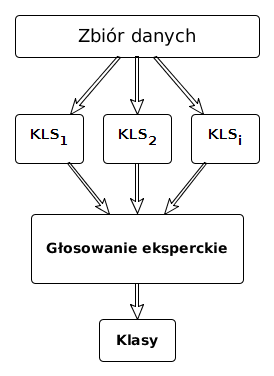
\includegraphics[width=\textwidth]{./images/klas_ekspercki.png}
	\caption{Schemat klasyfikatora eksperckiego. $KB_1..KB_i$ to klasyfikatory bazowe.}
	\label{fig:klasyfikator_ekspercki}
\end{figure}
Podstawowa wersja klasyfikatora znajduje się w pliku $classifiers/clf_expert.py$, a wersja ze sprawdzianem krzyżowym w pliku $classifiers/clf_expertCV.py$. Obsługa klasyfikatora odbywa się w takim sam sposób jak klasyfikatorów z biblioteki $scikit-learn$.
\subsection{Test klasyfikatora eksperckiego}
Test klasyfikatora eksperckiego przeprowadzono tak samo jak poprzednie. Został on powtórzony 10 razy, a wyniki zostały uśrednione. Test znajduje się w pliku $test_my_clfs/test_clf_expert.py$. Klasyfikator ekspercki został zbudowany z naiwnego klasyfikatora Bayesa, klasyfikatora kNN oraz drzewa decyzyjnego z maksymalną głębokością 3. Test przeprowadzono dla różnych funkcji wyłaniających ekspertów. CLFE to podstawowa wersja klasyfikatora, eksperci klasowi wyłaniani są na podstawie najlepszej precyzji. w CLFE F1 eksperci wyłaniani są na podstawie miary F-1 klas. Natomiast w CLFE G wyłonienie ekspertów odbywa się na podstawie miary G-mean. Skrót CV, oznacza wersję ze sprawdzianem krzyżowym. Wyniki zostały porównane do drzewa decyzyjnego (TREE) z maksymalną głębokością równą 3. Dokładność klasyfikacji (tabela \ref{ekspertacc}) oraz czułość klasy większościowej (tabela \ref{ekspertsens}) wzrosła dla większości zbiorów danych. Dla pozostałych zbiorów, wyniki były takie same jak drzewa decyzyjnego lub minimalnie niższe. Natomiast specyficzność klasy mniejszościowej (tabela \ref{ekspertspec}) oraz miara G-mean (tabeela \ref{ekspertgmean}) wzrosły lub utrzymały taką samą wartości jak drzewa decyzyjne w 21 zbiorach na 22. W wykrywaniu klasy mniejszościowej najlepsze okazały się klasyfikatory oparty o miarę F1 i G-mean. Pomiędzy wersją klasyfikatora ze sprawdzianem krzyżowym oraz bez, nie zauważono dużej różnicy w wynikach w większości zbiorów.
	\begin{table}[H]
		\tiny
		\begin{center}
			\resizebox{\textwidth}{!}{%
				\begin{tabular}{c|ccccccc}%
					Zbiór danych&TREE&CLFE&CLFE CV&CLFE F1&\specialcell{CLFE\\F1 CV}&CLFE G&\specialcell{CLFE\\G CV}\\%
					\hline%
					seeds&0.91&\textbf{0.92}&0.91&0.91&0.91&0.91&0.91\\%
					new\_thyroid&\textbf{0.97}&\textbf{0.97}&\textbf{0.97}&\textbf{0.97}&0.96&\textbf{0.97}&0.96\\%
					vehicle&0.9&0.9&0.9&\textbf{0.92}&\textbf{0.92}&\textbf{0.92}&0.9\\%
					ionosphere&0.86&0.88&\textbf{0.89}&0.86&0.87&0.86&0.87\\%
					vertebal&0.71&0.74&0.73&0.73&0.77&0.73&\textbf{0.78}\\%
					yeastME3&0.94&\textbf{0.95}&\textbf{0.95}&\textbf{0.95}&0.94&\textbf{0.95}&0.94\\%
					ecoli&0.86&0.85&0.85&0.87&0.87&\textbf{0.88}&0.76\\%
					bupa&0.65&\textbf{0.69}&0.68&0.68&0.67&0.68&0.6\\%
					horse\_colic&\textbf{0.86}&\textbf{0.86}&0.84&\textbf{0.86}&\textbf{0.86}&\textbf{0.86}&\textbf{0.86}\\%
					german&0.74&\textbf{0.76}&0.75&0.73&\textbf{0.76}&0.73&0.74\\%
					breast\_cancer&\textbf{0.73}&0.71&0.71&0.7&0.72&0.72&0.72\\%
					cmc&\textbf{0.78}&0.75&0.76&0.74&0.74&0.7&0.68\\%
					hepatitis&0.66&\textbf{0.68}&\textbf{0.68}&0.66&0.66&0.61&0.66\\%
					haberman&\textbf{0.75}&0.73&0.74&0.74&0.74&0.74&0.69\\%
					transfusion&0.68&\textbf{0.69}&0.68&0.68&\textbf{0.69}&0.68&\textbf{0.69}\\%
					car&0.69&0.89&\textbf{0.92}&\textbf{0.92}&\textbf{0.92}&0.89&0.89\\%
					glass&\textbf{0.82}&0.63&0.8&\textbf{0.82}&0.74&0.49&0.48\\%
					abalone16\_29&\textbf{0.94}&\textbf{0.94}&\textbf{0.94}&0.93&0.88&0.68&0.68\\%
					solar\_flare&\textbf{0.95}&0.81&0.94&\textbf{0.95}&0.87&0.65&0.65\\%
					heart\_cleveland&\textbf{0.86}&\textbf{0.86}&0.83&0.85&0.83&0.81&0.81\\%
					balance\_scale&\textbf{0.92}&\textbf{0.92}&\textbf{0.92}&\textbf{0.92}&\textbf{0.92}&\textbf{0.92}&\textbf{0.92}\\%
					postoperative&0.68&0.69&0.71&0.67&\textbf{0.72}&0.67&0.67\\%
				\end{tabular}}
				\caption{Dokładność klasyfikatora eksperckiego.}
				\label{ekspertacc}
			\end{center}
		\end{table}	
			\begin{table}[H]
				\tiny
				\begin{center}
					\resizebox{\textwidth}{!}{%
						\begin{tabular}{c|ccccccc}%
							Zbiór danych&TREE&CLFE&CLFE CV&CLFE F1&\specialcell{CLFE\\F1 CV}&CLFE G&\specialcell{CLFE\\G CV}\\%
							\hline%
							seeds&\textbf{0.92}&\textbf{0.92}&0.91&\textbf{0.92}&\textbf{0.92}&\textbf{0.92}&\textbf{0.92}\\%
							new\_thyroid&0.98&0.98&\textbf{0.99}&0.98&\textbf{0.99}&0.98&0.97\\%
							vehicle&0.89&0.89&0.89&\textbf{0.95}&\textbf{0.95}&\textbf{0.95}&0.89\\%
							ionosphere&0.92&0.97&\textbf{0.99}&0.92&0.93&0.92&0.93\\%
							vertebal&0.71&\textbf{0.72}&0.71&0.71&0.71&0.71&\textbf{0.72}\\%
							yeastME3&0.97&0.97&0.97&\textbf{0.98}&0.97&0.97&0.97\\%
							ecoli&0.9&0.88&0.86&\textbf{0.91}&0.89&0.9&0.77\\%
							bupa&0.72&0.77&0.81&0.81&0.72&\textbf{0.82}&0.63\\%
							horse\_colic&\textbf{0.92}&\textbf{0.92}&0.88&\textbf{0.92}&\textbf{0.92}&\textbf{0.92}&\textbf{0.92}\\%
							german&0.88&\textbf{0.89}&\textbf{0.89}&0.86&0.84&0.77&0.81\\%
							breast\_cancer&\textbf{0.92}&0.88&0.85&0.85&0.86&0.84&0.84\\%
							cmc&\textbf{0.9}&0.86&0.86&0.88&0.83&0.75&0.7\\%
							hepatitis&0.7&\textbf{0.73}&\textbf{0.73}&0.7&0.67&0.59&0.63\\%
							haberman&0.91&0.91&\textbf{0.93}&0.9&\textbf{0.93}&0.88&0.85\\%
							transfusion&0.76&\textbf{0.81}&0.8&0.8&\textbf{0.81}&0.76&0.8\\%
							car&0.71&0.89&\textbf{0.94}&\textbf{0.94}&\textbf{0.94}&0.89&0.89\\%
							glass&\textbf{0.88}&0.64&0.85&\textbf{0.88}&0.78&0.48&0.45\\%
							abalone16\_29&\textbf{1.0}&0.99&0.99&0.99&0.92&0.69&0.69\\%
							solar\_flare&\textbf{0.99}&0.83&0.98&0.98&0.88&0.64&0.64\\%
							heart\_cleveland&\textbf{0.97}&\textbf{0.97}&0.89&0.91&0.89&0.83&0.83\\%
							balance\_scale&\textbf{1.0}&\textbf{1.0}&\textbf{1.0}&\textbf{1.0}&\textbf{1.0}&\textbf{1.0}&\textbf{1.0}\\%
							postoperative&0.9&0.89&0.94&0.83&\textbf{0.95}&0.83&0.85\\%
						\end{tabular}}
						\caption{Czułość klasy większościowej dla klasyfikatora eksperckiego.}
						\label{ekspertsens}
					\end{center}
				\end{table}	
			\begin{table}[H]
				\tiny
				\begin{center}
					\resizebox{\textwidth}{!}{%
						\begin{tabular}{c|ccccccc}%
							Zbiór danych&TREE&CLFE&CLFE CV&CLFE F1&\specialcell{CLFE\\F1 CV}&CLFE G&\specialcell{CLFE\\G CV}\\%
							\hline%
							seeds&0.89&\textbf{0.91}&0.9&0.89&0.9&0.89&0.9\\%
							new\_thyroid&\textbf{0.87}&\textbf{0.87}&0.8&\textbf{0.87}&0.8&\textbf{0.87}&\textbf{0.87}\\%
							vehicle&\textbf{0.93}&\textbf{0.93}&\textbf{0.93}&0.84&0.84&0.84&\textbf{0.93}\\%
							ionosphere&0.75&0.71&0.71&0.75&\textbf{0.76}&0.75&\textbf{0.76}\\%
							vertebal&0.71&0.76&0.76&0.76&\textbf{0.9}&0.76&\textbf{0.9}\\%
							yeastME3&0.73&\textbf{0.77}&\textbf{0.77}&0.71&0.7&0.75&0.73\\%
							ecoli&0.49&0.6&0.71&0.51&0.63&\textbf{0.74}&0.69\\%
							bupa&0.55&0.57&0.5&0.5&\textbf{0.61}&0.48&0.57\\%
							horse\_colic&0.75&0.75&\textbf{0.78}&0.75&0.76&0.75&0.76\\%
							german&0.42&0.46&0.44&0.44&0.55&\textbf{0.62}&0.57\\%
							breast\_cancer&0.31&0.31&0.39&0.35&0.41&0.42&\textbf{0.44}\\%
							cmc&0.39&0.37&0.42&0.28&0.45&0.51&\textbf{0.61}\\%
							hepatitis&0.5&0.5&0.5&0.5&0.62&0.69&\textbf{0.78}\\%
							haberman&0.32&0.23&0.21&0.28&0.2&\textbf{0.35}&0.25\\%
							transfusion&\textbf{0.45}&0.32&0.3&0.31&0.3&0.41&0.35\\%
							car&0.32&\textbf{1.0}&0.43&0.43&0.43&\textbf{1.0}&\textbf{1.0}\\%
							glass&0.12&0.47&0.24&0.12&0.29&0.65&\textbf{0.82}\\%
							abalone16\_29&0.09&0.13&0.15&0.13&0.28&\textbf{0.58}&\textbf{0.58}\\%
							solar\_flare&0.12&0.44&0.12&0.09&0.63&\textbf{0.93}&\textbf{0.93}\\%
							heart\_cleveland&0.03&0.03&0.34&0.37&0.31&\textbf{0.63}&\textbf{0.63}\\%
							balance\_scale&\textbf{0.0}&\textbf{0.0}&\textbf{0.0}&\textbf{0.0}&\textbf{0.0}&\textbf{0.0}&\textbf{0.0}\\%
							postoperative&0.08&0.12&0.08&\textbf{0.21}&0.08&\textbf{0.21}&0.17\\%
						\end{tabular}}
						\caption{Specyficzność klasy mniejszościowej dla klasyfikatora eksperckiego.}
						\label{ekspertspec}
					\end{center}
				\end{table}	
			\begin{table}[H]
				\tiny
				\begin{center}
					\resizebox{\textwidth}{!}{%
						\begin{tabular}{c|ccccccc}%
							Zbiór danych&TREE&CLFE&CLFE CV&CLFE F1&\specialcell{CLFE\\F1 CV}&CLFE G&\specialcell{CLFE\\G CV}\\%
							\hline%
							seeds&0.9&\textbf{0.92}&0.91&0.9&0.91&0.9&0.91\\%
							new\_thyroid&\textbf{0.92}&\textbf{0.92}&0.89&\textbf{0.92}&0.89&\textbf{0.92}&\textbf{0.92}\\%
							vehicle&\textbf{0.91}&\textbf{0.91}&\textbf{0.91}&0.89&0.89&0.89&\textbf{0.91}\\%
							ionosphere&0.83&0.83&\textbf{0.84}&0.83&\textbf{0.84}&0.83&\textbf{0.84}\\%
							vertebal&0.71&0.74&0.74&0.74&\textbf{0.8}&0.74&\textbf{0.8}\\%
							yeastME3&0.84&\textbf{0.86}&\textbf{0.86}&0.83&0.82&0.85&0.84\\%
							ecoli&0.66&0.73&0.79&0.69&0.75&\textbf{0.82}&0.73\\%
							bupa&0.63&\textbf{0.67}&0.64&0.63&0.66&0.63&0.6\\%
							horse\_colic&\textbf{0.83}&\textbf{0.83}&\textbf{0.83}&\textbf{0.83}&\textbf{0.83}&\textbf{0.83}&\textbf{0.83}\\%
							german&0.61&0.64&0.63&0.61&0.68&\textbf{0.69}&0.68\\%
							breast\_cancer&0.53&0.52&0.57&0.55&0.59&\textbf{0.6}&\textbf{0.6}\\%
							cmc&0.59&0.56&0.6&0.49&0.61&0.62&\textbf{0.65}\\%
							hepatitis&0.59&0.6&0.6&0.59&0.65&0.63&\textbf{0.7}\\%
							haberman&0.54&0.46&0.44&0.5&0.43&\textbf{0.55}&0.46\\%
							transfusion&\textbf{0.59}&0.51&0.49&0.5&0.49&0.56&0.53\\%
							car&0.48&\textbf{0.94}&0.64&0.63&0.63&\textbf{0.94}&\textbf{0.94}\\%
							glass&0.32&0.55&0.45&0.32&0.48&0.56&\textbf{0.61}\\%
							abalone16\_29&0.3&0.35&0.39&0.35&0.5&\textbf{0.63}&\textbf{0.63}\\%
							solar\_flare&0.34&0.61&0.34&0.3&0.74&\textbf{0.77}&\textbf{0.77}\\%
							heart\_cleveland&0.17&0.17&0.55&0.58&0.53&\textbf{0.72}&\textbf{0.72}\\%
							balance\_scale&\textbf{0.0}&\textbf{0.0}&\textbf{0.0}&\textbf{0.0}&\textbf{0.0}&\textbf{0.0}&\textbf{0.0}\\%
							postoperative&0.27&0.33&0.28&\textbf{0.42}&0.28&\textbf{0.42}&0.38\\%
						\end{tabular}}
						\caption{Miara G-mean dla klasyfikatora eksperckiego.}
						\label{ekspertgmean}
					\end{center}
				\end{table}	
\section{Meta-klasyfikator}
Algorytm klasyfikacji danych wybiera się w zależności od charakterystyki i rodzaju danych. Budowany meta-klasyfikator miał osiągać dobre wyniki dla różnych zbiorów danych. 
Celem budowanego meta-klasyfikatora miało być stworzenie uniwersalnego 
\begin{figure}[H]
	\centering
	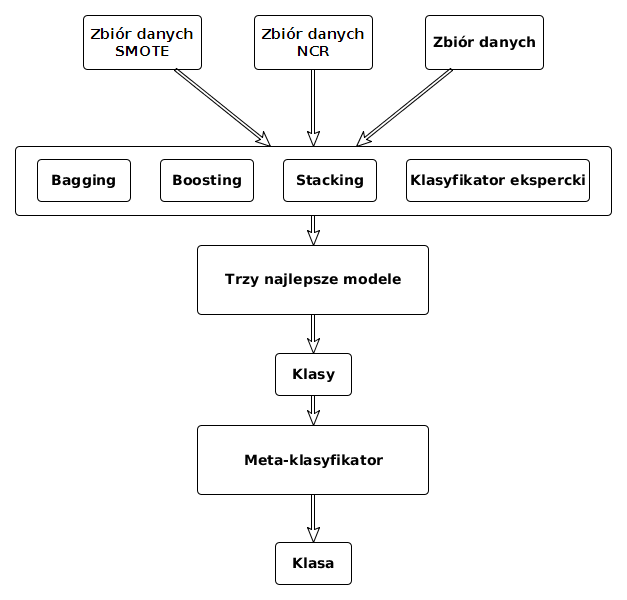
\includegraphics[width=\textwidth]{./images/metaklas.png}
	\caption{Projekt meta-klasyfikatora}
	\label{fig:metaklasmoj}
\end{figure}
\subsection{Testy}